\documentclass[11pt]{article}
\usepackage[top=1.00in, bottom=1.0in, left=1.1in, right=1.1in]{geometry}
\renewcommand{\baselinestretch}{1.1}
\usepackage{graphicx}
\usepackage{natbib}
\usepackage{gensymb}
\usepackage{amsmath}
\usepackage{lineno}
\usepackage{xr-hyper}
\usepackage{longtable}
% \usepackage{tabularx}
% \usepackage{array}

\externaldocument{limitingcues}

\def\labelitemi{--}
\parindent=0pt

\usepackage{Sweave}
\begin{document}
\renewcommand{\thetable}{S\arabic{table}}
\renewcommand{\thefigure}{S\arabic{figure}}

\bibliographystyle{/Users/Lizzie/Documents/EndnoteRelated/Bibtex/styles/besjournals}
\renewcommand{\refname}{\CHead{}}
\begin{flushright}
Version dated: \today
\end{flushright}
\bigskip
\medskip
\begin{center}

\noindent{\Large {\bf Limiting cues: How spring warming, winter chilling and daylength will shape climate change responses}}\\ 
\bigskip

\noindent {\normalsize \sc
The lab as it was in 2017$^{1,2}$}\\ % Ailene, Cat, Dan, Lizzie, Nacho
\noindent {\small \it
$^1$ Arnold Arboretum of Harvard University, 1300 Centre Street, Boston, Massachusetts, 02131, USA\\
$^2$ Organismic \& Evolutionary Biology, Harvard University, 26 Oxford Street, Cambridge, Massachusetts, 02138, USA\\
$^3$ Forest \& Conservation Sciences, Faculty of Forestry, University of British Columbia, 2424 Main Mall, Vancouver, BC V6T 1Z4}\\
\end{center}


\section{Overview of OSPREE}
Studies versus papers ... how many crops versus wild species ....

% Add info on ..
% earliest and latest studies
% types of events
% cleaning is hard, that's why the data are old?
% table of studies

We built the Observed Spring Phenology Responses in Experimental Environments (OSPREE) database, by searching  both ISI Web of Science and Google Scholar  the following terms: 
\begin{enumerate}
\item TOPIC = (budburst OR leaf-out) AND (photoperiod or daylength) AND temperature*, which yielded 85 publications
\item TOPIC = (budburst OR leaf-out) AND dorman*, which yielded 193 publications
\end{enumerate}

49 papers in budburst table ... here we present 84 or which 21 are focused on crops (\emph{Actinidia deliciosa, Malus domestica, Vitis vinifera, Ribes nigrum, Vaccinium ashei, Vaccinium corymbosum, Prunus persica}). Studies spanned a variety of plant materials, though studies on `seedlings' (51 studies) and `cuttings' (55 studies) were most common. 

\section{Trends in experimental treatments over space}


The actual cues studied varied across latitude with a general trend toward examining more extreme values at higher latitudes. Thus, forcing and chilling treatments decline 0.1$\degree$C per 1 $\degree$ latitude (for forcing, min is -0.1, for max it's -0.06, see Fig \ref{fig:lat}; for chilling it's -0.06 for min and -0.09 for max); and the maximum studied photoperiod increases with latitude (0.09 hr per degree $\degree$ latitude). 

\section{Comparing experimental treatments to forecasted trends}
% studydesignplots.R

 Treatment differences were calculated as the differences within varying forcing and chilling treatments within a single study (e.g., a study with a 1 and 4$\degree$C chilling treatment would yield a value of 3$\degree$C). 
 
 19 studies for \emph{Fagus sylvatica}  and 17 for \emph{Betula pendula},
 
 136 total studies
 
\newpage
\section{References}
\bibliography{..//..//refs/ospreebibplus}

\newpage
\section* {Supplemental Tables}
\begin{footnotesize} 

% latex table generated in R 3.5.1 by xtable 1.8-3 package
% Wed Mar 31 10:22:50 2021
\begingroup\footnotesize
\begin{longtable}{p{0.15\textwidth}p{0.50\textwidth}}
\caption{\textbf{Dataset names and references for papers in the OSPREE database.}} \\ 
  \hline
Dataset & Reference \\ 
  \hline \endhead  \hline
ashby62 & \citep{Ashby:1962aa} \\ 
  basler12 & \citep{Basler:2012} \\ 
  basler14 & \citep{Basler:2014aa} \\ 
  biasi12 & \citep{Biasi:2012} \\ 
  boyer & \citep{Boyer:1986} \\ 
  caffarra11a & \citep{Caffarra:2011a} \\ 
  caffarra11b & \citep{Caffarra:2011b} \\ 
  calme94 & \citep{Calme:1994aa} \\ 
  campbell75 & \citep{Campbell:1975aa} \\ 
  cannell83 & \citep{Cannell:1983} \\ 
  charrier11 & \citep{Charrier:2011aa} \\ 
  chavarria09 & \citep{Chavarria:2009aa} \\ 
  cook00b & \citep{Cook:2000aa} \\ 
  cook05 & \citep{Cook:2005aa} \\ 
  cronje03 & \citep{Cronje:2003aa} \\ 
  dantec14 & \citep{Dantec:2014aa} \\ 
  devries82 & \citep{DeVries:1982aa} \\ 
  falusi03 & \citep{Falusi:2003aa} \\ 
  falusi90 & \citep{Falusi:1990aa} \\ 
  falusi96 & \citep{Falusi:1996aa} \\ 
  falusi97 & \citep{Falusi:1997aa} \\ 
  fu13 & \citep{Fu:2013aa} \\ 
  gansert02 & \citep{Gansert:2002aa} \\ 
  ghelardini10 & \citep{Ghelardini:2010aa} \\ 
  gianfagna85 & \citep{Gianfagna:1985aa} \\ 
  gomory15 & \citep{Gomory:2015aa} \\ 
  granhus09 & \citep{Granhus:2009aa} \\ 
  guak98 & \citep{Guak:1998aa} \\ 
  guerriero90 & \citep{guerriero:1990} \\ 
  gunderson12 & \citep{Gunderson:2012aa} \\ 
  hawerroth13 & \citep{Hawerroth:2013aa} \\ 
  hawkins12 & \citep{Hawkins:2012} \\ 
  heide03 & \citep{Heide:2003aa} \\ 
  heide05 & \citep{Heide:2005aa} \\ 
  heide08 & \citep{Heide:2008aa} \\ 
  heide11 & \citep{Heide:2011aa} \\ 
  heide12 & \citep{Heide:2012aa} \\ 
  heide15 & \citep{Heide:2015aa} \\ 
  heide93 & \citep{Heide:1993} \\ 
  heide93a & \citep{Heide:1993a} \\ 
  howe95 & \citep{Howe:1995aa} \\ 
  jones12 & \citep{Jones:2012} \\ 
  junttila12 & \citep{Junttila:2012aa} \\ 
  karlsson03 & \citep{Karlsson:2003aa} \\ 
  lamb37 & \citep{Lamb:1948aa} \\ 
  laube14a & \citep{Laube:2014a} \\ 
  laube14b & \citep{Laube:2014b} \\ 
  li05 & \citep{Li:2005aa} \\ 
  linkosalo06 & \citep{Linkosalo:2006aa} \\ 
  man10 & \citep{Man:2010aa} \\ 
  manson91 & \citep{Manson:1991aa} \\ 
  morin10 & \citep{Morin:2010aa} \\ 
  myking95 & \citep{Myking:1995} \\ 
  myking97 & \citep{Myking:1997aa} \\ 
  myking98 & \citep{Myking:1998aa} \\ 
  nienstaedt66 & \citep{Nienstaedt:1966aa} \\ 
  nishimoto95 & \citep{Nishimoto:1994aa} \\ 
  okie11 & \citep{Okie:2011aa} \\ 
  pagter15 & \citep{Pagter:2015} \\ 
  partanen01 & \citep{Partanen:2001aa} \\ 
  partanen05 & \citep{Partanen:2005aa} \\ 
  partanen98 & \citep{Partanen:1998aa} \\ 
  pettersen71 & \citep{Pettersen:1972aa} \\ 
  pop2000 & \citep{Pop:2000aa} \\ 
  ramos99 & \citep{ramos:1999} \\ 
  rinne94 & \citep{Rinne:1994} \\ 
  rinne97 & \citep{Rinne:1997aa} \\ 
  ruesink98 & \citep{Ruesink:1998aa} \\ 
  sanz-perez09 & \citep{Sanz-Perez:2009aa} \\ 
  sanzperez10 & \citep{Sanz-Perez:2010aa} \\ 
  schnabel87 & \citep{Schnabel:1987aa} \\ 
  skre08 & \citep{Skre:2008aa} \\ 
  skuterud94 & \citep{Skuterud:1994aa} \\ 
  sogaard08 & \citep{Sogaard:2008aa} \\ 
  sonsteby13 & \citep{Sonsteby:2013aa} \\ 
  sonsteby14 & \citep{Sonsteby:2014aa} \\ 
  spiers74 & \citep{Spiers:1974aa} \\ 
  swartz81 & \citep{Swartz:1981aa} \\ 
  thielges75 & \citep{Thielges:1976aa} \\ 
  viheraaarnio06 & \citep{Vihera-Aarnio:2006aa} \\ 
  webb78 & \citep{Webb:1977} \\ 
  worrall67 & \citep{Worrall:1967aa} \\ 
  yazdaniha64 & \citep{Yazdaniha:1967aa} \\ 
  zohner16 & \citep{zohner2016} \\ 
  \hline
\label{tab:ref}
\end{longtable}
\endgroup\end{footnotesize} 

\pagebreak

\begin{figure}[t!]
\centering
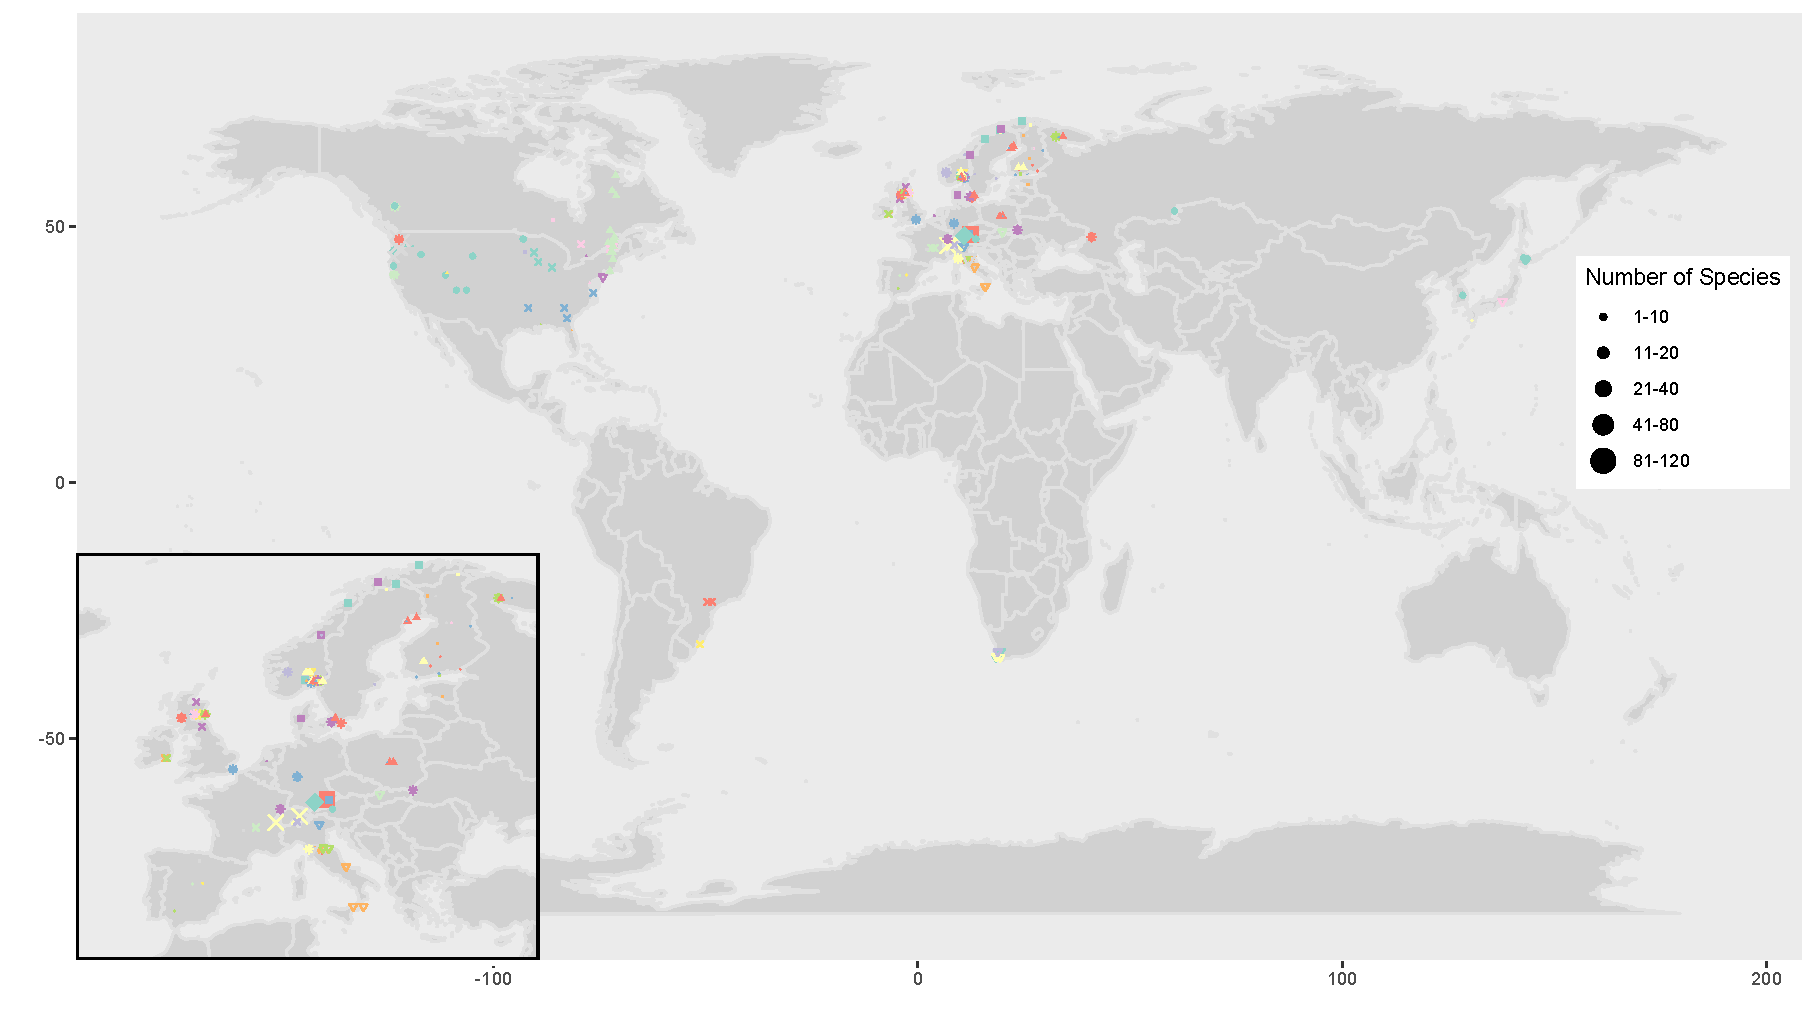
\includegraphics[width=1\textwidth]{..//..//analyses/limitingcues/figures/maps/map_studyspp.pdf}
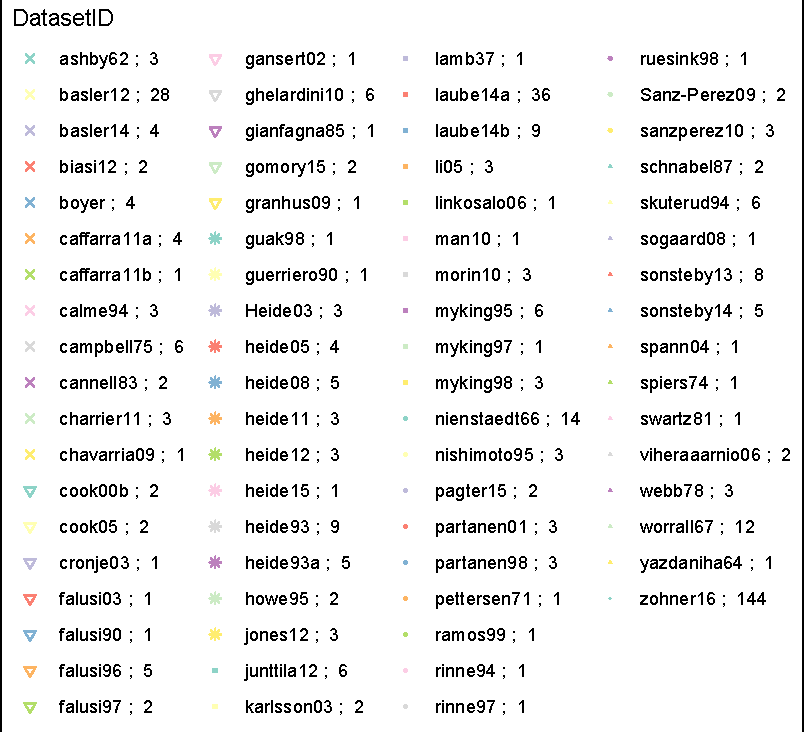
\includegraphics[width=0.5\textwidth]{..//..//analyses/limitingcues/figures/maps/map_studyspp_legend.pdf}
\caption{We review seven decades of controlled environment studies, from \citet{Lamb:1948aa} to \citet{zohner2016}, conducted across the globe generally on 1-3 species in each experiment (size of circles and exact number of species given after each each study). }
  \label{fig:datamap} % Ailene: This figure is nice. i would say, though, that i don't find the size of the shapes to be particularly easy to interpret. seeing the numbers next to each study is a much more effective at showing that most studies have fewer than 5 spp.
\end{figure}


\begin{figure}[t!]
\centering
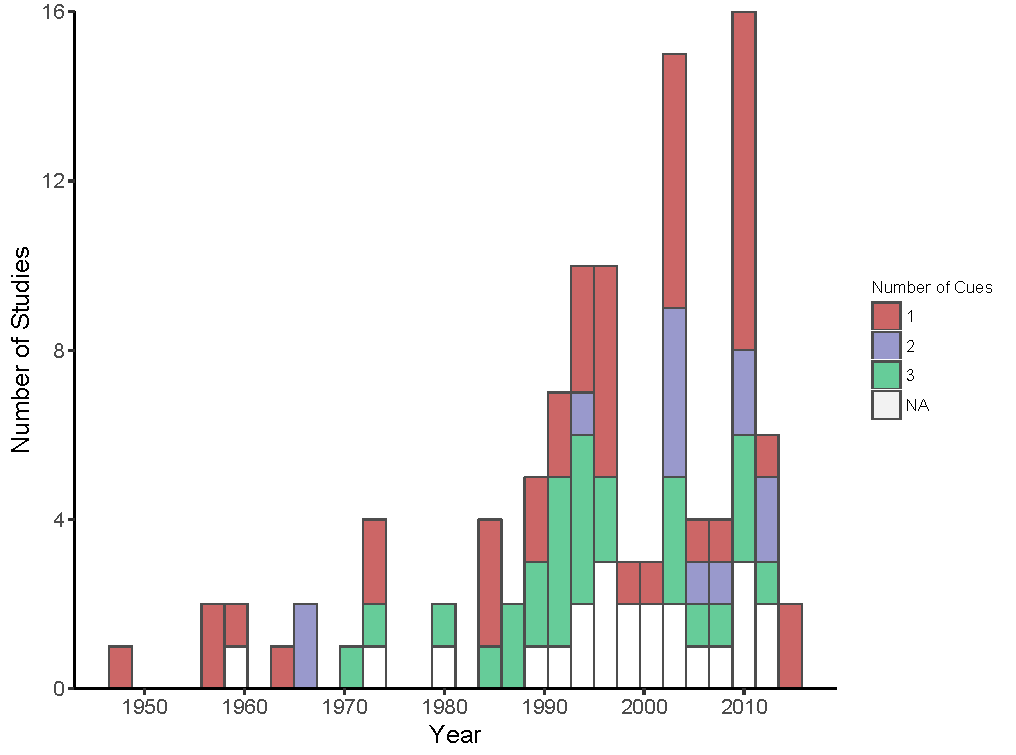
\includegraphics[width=0.8\textwidth]{..//..//analyses/limitingcues/figures/studyyearcues.pdf}
\caption{Cues manipulated over time.}
  \label{fig:ts}
\end{figure}


\begin{figure}[t!]
\centering
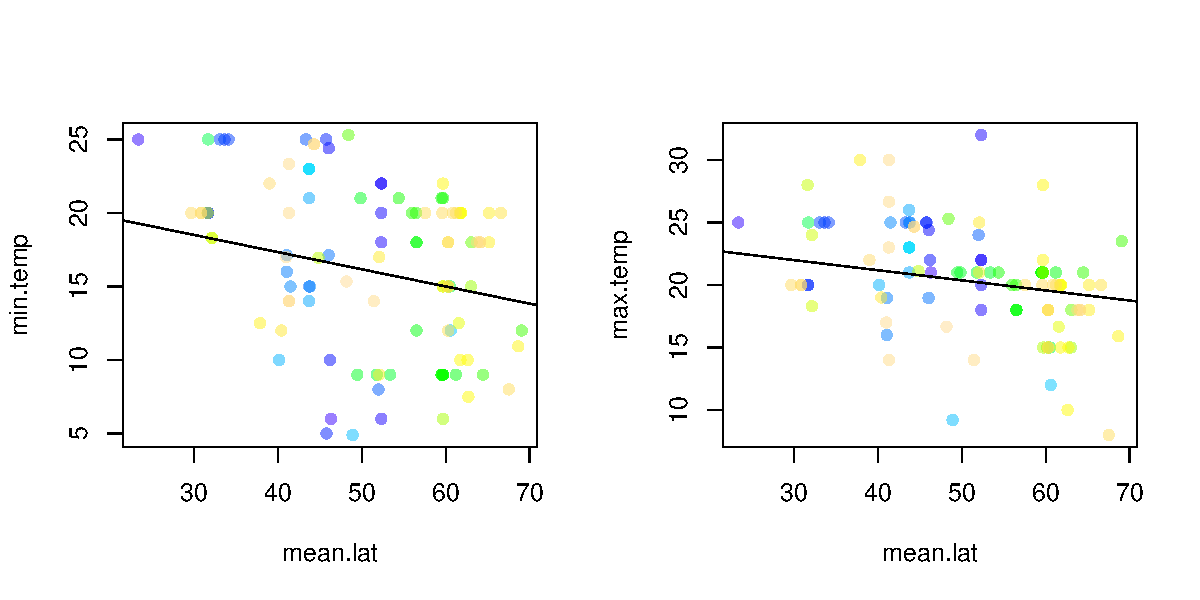
\includegraphics[width=1\textwidth]{..//..//analyses/limitingcues/figures/tempxlatminmaxcorr.pdf}
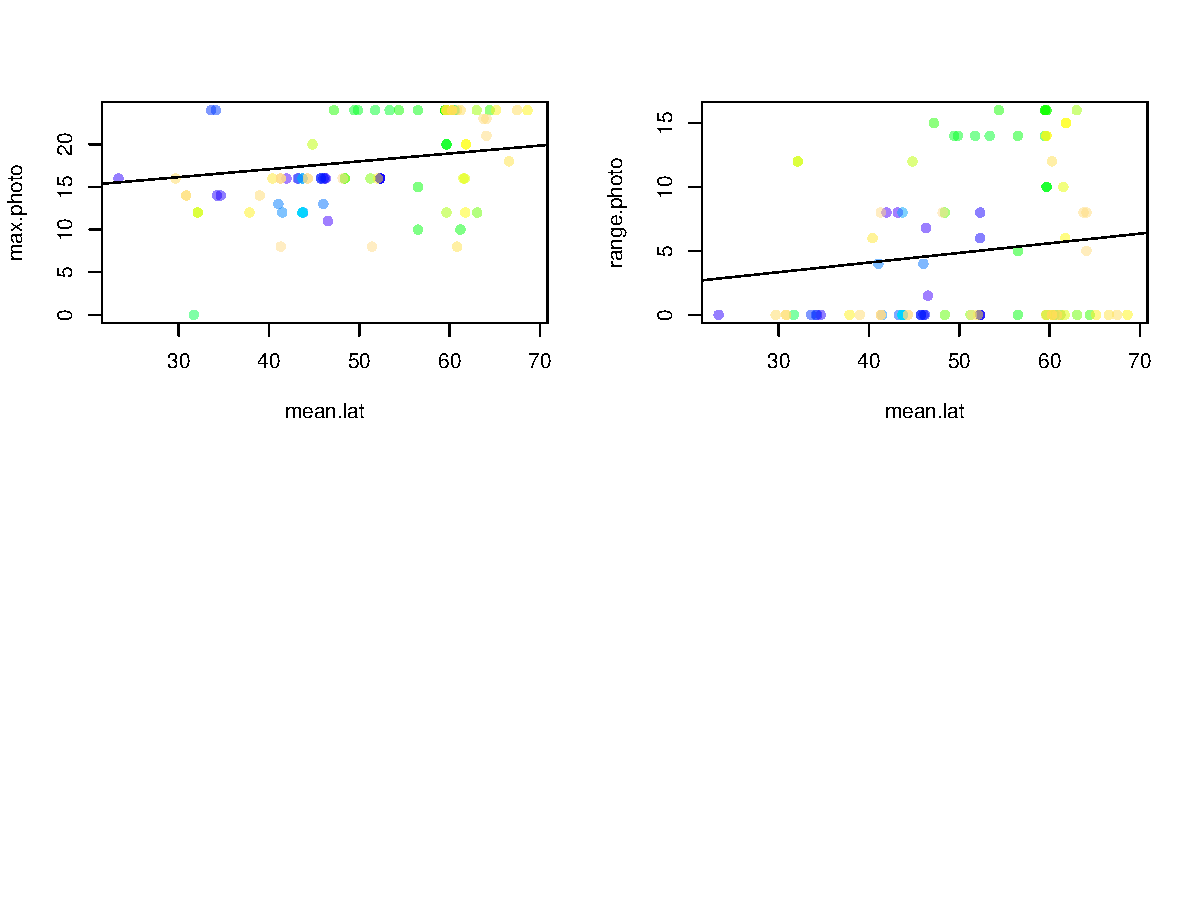
\includegraphics[width=1\textwidth]{..//..//analyses/limitingcues/figures/photoxlatcorr2plots.pdf}
\caption{Some correlations with latitude plots.}
  \label{fig:lat}
\end{figure}


\end{document}





